% Chapter 4
% Implementação

\chapter{Implementação}
\label{chap:Chapter4}

Este capítulo descreve como a \gls{pipeline} e o instrumento de recolha foram construídos. A definição operacional da ambivalência, o desenho factorial e o protocolo humano estão no Capítulo~\ref{chap:Chapter3}; aqui fica a realização, código, \textit{prompts}, persistência e exportação. A geração corre em Python, com Hugging Face Transformers, sem \glspl{api} proprietárias \parencite{Wolf2020Transformers}. O código e os artefactos de replicação estão em \url{https://github.com/marcelobarrosow/isep-mestrado-dissertacao}.

%----------------------------------------------------------------------------------------

\section{Arquitectura da solução}
\label{sec:impl_arquitectura}

A implementação separa dois subsistemas, ligados por artefactos em disco, não por uma \gls{api} em tempo de execução. Lê os 12 estímulos, deriva o sinal de \gls{ambivalenciaemocional} e produz as 96 células. A recolha corre em \gls{php} e MariaDB. Importa o catálogo bilingue, aplica a rotação cega e exporta as classificações Likert. A análise estatística lê o \gls{csv} público e não chama os modelos. O lote avaliado no repositório de replicação é \texttt{data/all\_results.json}; a cópia arquivada nesta dissertação é \texttt{appendices/data/all\_results.json}. Regenerar células em \texttt{pipeline/outputs/} não substitui esse lote nem reproduz a avaliação humana.

O repositório organiza-se em três pastas. O código complementa esta descrição e não a substitui.

\begin{verbatim}
pipeline/   geração (pipeline.py + módulos) e scripts de análise
site/       questionário PHP/MariaDB (páginas + lib/)
data/       artefactos canónicos (JSON, CSV, codebook)
\end{verbatim}

A Figura~\ref{fig:sistema_contexto} situa os actores e o contrato por ficheiro. O autor corre a geração e a administração. O participante só vê o instrumento. Os modelos Hugging Face são carregados localmente pelo gerador. O questionário nunca os invoca.

\begin{figure}[ht]
\centering
\begin{tikzpicture}[
  node distance=0.5cm and 0.7cm,
  box/.style={draw, rounded corners=2pt, align=center, font=\small, inner sep=4pt, minimum height=0.85cm},
  act/.style={draw, align=center, font=\small, inner sep=4pt, minimum height=0.7cm},
  arr/.style={-{Stealth}, thick}
]
\node[act] (autor) {Autor};
\node[act, right=3.2cm of autor] (part) {Participante};
\node[box, below=of autor] (gen) {Geração\\Python (\texttt{pipeline/})};
\node[box, below=of part] (site) {Recolha\\PHP + MariaDB};
\node[act, left=0.6cm of gen] (hf) {Hugging Face\\(local)};
\node[box, below=1.15cm of gen, xshift=1.7cm] (data) {\texttt{data/} com JSON, CSV bilingue\\e classificações públicas};
\node[box, below=of data] (ana) {Análise\\(\texttt{analyze\_survey\_mixed.py})};
\draw[arr] (autor) -- (gen);
\draw[arr] (hf) -- (gen);
\draw[arr] (part) -- (site);
\draw[arr] (gen.south) -- ++(0,-0.4) -| (data.north);
\draw[{Stealth}-{Stealth}, thick] (site.south) -- ++(0,-0.45) -| (data.north east);
\draw[arr] (data) -- (ana);
\end{tikzpicture}
\caption[Contexto do sistema.]{Contexto do sistema. Geração, recolha e análise comunicam por ficheiros, sem \acrshort{api} em runtime.}
\label{fig:sistema_contexto}
\end{figure}

O analisador emocional, em \texttt{emotion\_analyzer.py}, usa \path{SamLowe/roberta-base-go_emotions} e deriva a \gls{ambivalenciaemocional} com limiar \(\tau = 0{,}10\) \parencite{Demszky2020GoEmotions}. O gerador âncora da época sob avaliação é carregado em \texttt{generator.py} a partir do identificador Hugging Face.

As condições experimentais partilham a mesma intenção de \textit{prompt}.
\begin{itemize}
 \item Na \textit{baseline}, a instrução é de assistente conversacional, sem metadados afectivos.
 \item Na \gls{condicaopipeline}, a mesma instrução inclui o sinal de ambivalência (emoção positiva e negativa dominantes), com a regra de não falar da análise.
\end{itemize}

DialoGPT e BlenderBot usam geradores adaptados às arquitecturas (\textit{causal} e \textit{seq2seq}) \parencite{Zhang2020DialoGPT, Roller2021BlenderBot}. Phi-3-mini e Qwen2.5-3B usam os modelos de conversa no formato de instrução do próprio Hugging Face \parencite{Abdin2024Phi3, Yang2025Qwen25}. O tecto de tokens novos está fixo no protocolo, para respostas curtas (duas a quatro frases nas âncoras instruct), alinhado aos \textit{prompts} da Secção~\ref{sec:impl_prompts}. Os parâmetros de descodificação registados nas 96 células constam da mesma secção.

A pipeline de geração está em módulos com responsabilidades distintas. O \gls{cli}, em \texttt{pipeline.py}, orquestra o lote, com pré-filtro de ambivalência, um gerador por época, células já no disco e \textit{merge}. A orquestração de \textit{uma} célula vive em \texttt{cells.py} (\texttt{run\_cell}). A Figura~\ref{fig:pipeline_componentes} mostra as chamadas. \texttt{prompts.py} não fala com o modelo. \texttt{quality.py} não gera texto. \texttt{generator.py} recebe o \textit{prompt} já formatado. A condição experimental, \textit{baseline} ou \gls{condicaopipeline}, escolhe-se dentro de \texttt{run\_cell}, não no gerador.

\begin{figure}[ht]
\centering
\resizebox{\linewidth}{!}{%
\begin{tikzpicture}[
  box/.style={draw, rounded corners=2pt, align=center, font=\small\ttfamily, inner sep=4pt, minimum height=0.75cm},
  ext/.style={draw, align=center, font=\small, inner sep=4pt, minimum height=0.75cm},
  arr/.style={-{Stealth}, thick}
]
\node[box] (cli) at (0,2.6) {pipeline.py};
\node[box] (cells) at (0,1.5) {cells.py};
\node[box] (ea) at (-6.2,0) {emotion\_analyzer.py};
\node[box] (pr) at (-2.1,0) {prompts.py};
\node[box] (gen) at (2.1,0) {generator.py};
\node[box] (qa) at (6.0,0) {quality.py};
\node[ext] (goe) at (-6.2,-1.2) {GoEmotions\\(CPU)};
\node[ext] (hf) at (2.1,-1.2) {Âncora \(E_i\)};
\node[ext] (json) at (0,-2.5) {JSON da célula};
\draw[arr] (cli) -- (cells);
\draw[arr] (cells.south west) -- (ea.north);
\draw[arr] (cells.south) -- (pr.north);
\draw[arr] (cells.south) -- (gen.north);
\draw[arr] (cells.south east) -- (qa.north);
\draw[arr] (ea) -- (goe);
\draw[arr] (gen) -- (hf);
\draw[arr] (cells.south) -- (json.north);
\end{tikzpicture}%
}
\caption[Componentes da pipeline de geração.]{Componentes da pipeline de geração. O \acrshort{cli} orquestra o lote e grava o JSON. \texttt{run\_cell} produz o registo e chama analisador, \textit{prompts}, gerador e \acrshort{qa}.}
\label{fig:pipeline_componentes}
\end{figure}

\subsection{Fluxo de processamento}
\label{subsec:impl_fluxo}

A Figura~\ref{fig:pipeline_fluxo} resume o que acontece ao texto. O estímulo em inglês entra no GoEmotions \parencite{Demszky2020GoEmotions}, que devolve um vector de scores. A regra \(\tau = 0{,}10\) separa emoções positivas e negativas, escolhe as dominantes de cada valência e marca ambivalência se ambas ultrapassam o limiar. Consoante a condição, constrói-se o \textit{prompt} baseline ou o \textit{prompt} com contexto. O adaptador da âncora \(E_i\) formata essa entrada à arquitectura do modelo. O gerador produz a resposta. A célula é serializada em \gls{json}, exportada para \gls{csv} bilingue, importada para o questionário (MariaDB) e, no fim da recolha, exportada de novo para os scripts de análise do Capítulo~\ref{chap:Chapter5}.

\begin{figure}[ht]
\centering
\begin{tikzpicture}[
  node distance=0.55cm and 0.4cm,
  box/.style={draw, rounded corners=2pt, align=center, font=\small, inner sep=4pt, minimum height=0.85cm},
  arr/.style={-{Stealth}, thick}
]
\node[box] (stim) {Estímulo\\(texto EN)};
\node[box, right=of stim] (goe) {GoEmotions\\multilabel};
\node[box, right=of goe] (tau) {Sinal\\(\(\tau=0{,}10\))};
\node[box, below=of tau] (cond) {Condição\\baseline / pipeline};
\node[box, left=of cond] (prompt) {\textit{Prompt}\\por arquitectura};
\node[box, left=of prompt] (gen) {Gerador\\âncora \(E_i\)};
\node[box, below=of gen] (out) {\acrshort{json} / \acrshort{csv}\\96 células};
\draw[arr] (stim) -- (goe);
\draw[arr] (goe) -- (tau);
\draw[arr] (tau) -- (cond);
\draw[arr] (cond) -- (prompt);
\draw[arr] (prompt) -- (gen);
\draw[arr] (gen) -- (out);
\end{tikzpicture}
\caption{Fluxo de dados da pipeline, do estímulo ao JSON da célula, condicionado pelo sinal de ambivalência.}
\label{fig:pipeline_fluxo}
\end{figure}

\subsection{Chamadas de uma célula}
\label{subsec:impl_chamadas}

O lote (\texttt{main} em \texttt{pipeline.py}) percorre os 12 estímulos, as quatro épocas e as duas condições. O Algoritmo~\ref{alg:lote} resume essa orquestração: pré-filtro de ambivalência, um gerador por época, salto das células já gravadas, \texttt{run\_cell} e \texttt{merge\_results}.

\begin{algorithm}[H]
\caption{Geração do lote (\texttt{main} em \texttt{pipeline.py}).}
\label{alg:lote}
\begin{algorithmic}[1]
\Require estímulos, épocas E1--E4, condições \{\textit{baseline}, \textit{pipeline}\}, \(\tau=0{,}10\)
\Ensure células em disco e CSV de itens
\State carregar o analisador GoEmotions
\ForAll{estímulo \(t\)}
  \If{\(t\) não é ambivalente sob \(\tau\)}
    \State descartar \(t\)
  \EndIf
\EndFor
\ForAll{época \(E_i\)}
  \State instanciar \texttt{HFGenerator}(\(E_i\))
  \ForAll{estímulo \(t\) retido \(\times\) condição \(c\)}
    \If{a célula já existe em disco}
      \State saltar
    \Else
      \State \(\textit{row} \gets \mathrm{run\_cell}(t, c)\)
      \State gravar JSON da célula
    \EndIf
  \EndFor
  \State descarregar o gerador
\EndFor
\State \texttt{merge\_results}; exportar CSV de itens
\end{algorithmic}
\end{algorithm}

Uma célula isolada, com o analisador e o gerador já carregados, segue outro caminho. A Figura~\ref{fig:run_cell_seq} mostra as chamadas entre \texttt{cells.py}, o analisador, os \textit{prompts}, o gerador e a \gls{qa}.

\begin{figure}[H]
\centering
\resizebox{\linewidth}{!}{%
\begin{tikzpicture}[
  font=\scriptsize,
  arr/.style={-{Stealth}, thick},
  lab/.style={font=\scriptsize, inner sep=1pt, fill=white}
]
\foreach \x/\lab in {0/cells.py, 2.8/EmotionAnalyzer, 5.6/prompts.py, 8.4/HFGenerator, 11.2/quality.py} {
  \node[font=\scriptsize\ttfamily, align=center, anchor=south, text width=2.5cm] at (\x, 0.15) {\lab};
  \draw[dashed] (\x, 0) -- (\x, -11.2);
}
% 1. analyze
\draw[arr] (0,-0.7) -- node[lab, above] {\texttt{analyze}} (2.8,-0.7);
% 2. classify on the analyzer lifeline
\draw[arr] (2.8,-1.3) -- ++(1.15,0) -- ++(0,-0.55) -- node[lab, below] {\texttt{classify}+\texttt{build\_context}} ++(-1.15,0);
% 3. context back
\draw[arr] (2.8,-2.4) -- node[lab, above] {\texttt{EmotionalContext}} (0,-2.4);
% 4. prompt
\draw[arr] (0,-3.2) -- node[lab, above] {\texttt{build\_*\_prompt}} (5.6,-3.2);
\draw[arr] (5.6,-3.9) -- node[lab, above] {\textit{prompt}} (0,-3.9);
% QA loop
\draw[thick] (-0.85,-4.55) rectangle (12.05,-9.15);
\node[font=\scriptsize, anchor=south west] at (-0.75,-4.5) {ciclo \acrshort{qa} (até aceitar)};
\draw[arr] (0,-5.2) -- node[lab, above] {\texttt{generate}} (8.4,-5.2);
\draw[arr] (8.4,-6.1) -- node[lab, above] {resposta} (0,-6.1);
\draw[arr] (0,-7.1) -- node[lab, above] {\texttt{issues}} (11.2,-7.1);
\draw[arr] (11.2,-8.1) -- node[lab, above] {flags} (0,-8.1);
% persist
\node[lab, anchor=west] at (0.2,-10.3) {devolver o registo (o \acrshort{cli} grava, tentativas não contadas)};
\draw[arr] (0,-9.7) -- (0,-10.15);
\end{tikzpicture}%
}
\caption[Chamadas de \texttt{run\_cell}.]{Chamadas de \texttt{run\_cell}, com análise, construção do \textit{prompt}, geração e ciclo de \acrshort{qa} até aceitar a resposta.}
\label{fig:run_cell_seq}
\end{figure}

O analisador classifica o enunciado e deriva o contexto (\(\tau = 0{,}10\)). Se a condição é \textit{baseline}, chama-se \texttt{build\_direct\_prompt}. Se é \textit{pipeline}, chama-se \texttt{build\_contextual\_prompt}. O argumento \texttt{arch} vem do gerador (\texttt{causal\_dialogue}, \texttt{seq2seq} ou \texttt{chat}). Os identificadores canónicos do questionário, do tipo \texttt{s01\_\_E1\_\_baseline}, são produzidos por \texttt{sync\_study\_artifacts.py}. O CSV cego opcional de \texttt{export\_blind\_csv} usa \texttt{item\_001}, \texttt{item\_002}, \(\ldots\), e o instrumento não o importa. O Algoritmo~\ref{alg:run_cell} condensa o mesmo ciclo: analisar, construir o \textit{prompt} da condição, gerar e repetir até a \gls{qa} aceitar.

\begin{algorithm}[H]
\caption{Geração de uma célula (\texttt{run\_cell}).}
\label{alg:run_cell}
\begin{algorithmic}[1]
\Require estímulo \(t\), condição \(c\), analisador, gerador âncora
\Ensure registo da célula (JSON)
\State \(\textit{ctx} \gets \mathrm{analyze}(t)\) \Comment{\texttt{EmotionAnalyzer}, \(\tau=0{,}10\)}
\If{\(c = \textit{baseline}\)}
  \State \(\textit{prompt} \gets \mathrm{build\_direct\_prompt}(t, \textit{arch})\)
\Else
  \State \(\textit{prompt} \gets \mathrm{build\_contextual\_prompt}(t, \textit{ctx}, \textit{arch})\)
\EndIf
\State \(\textit{attempt} \gets 0\)
\State \(\textit{issues} \gets \{\texttt{empty}\}\)
\While{\(\textit{issues} \neq \emptyset\)}
  \State \(\mathrm{set\_seed}(42 + \textit{attempt}\times 17 + \textit{cell\_salt})\) \Comment{não constitui amostragem (guloso/beam)}
  \State \(\textit{resp} \gets \mathrm{generate}(\textit{prompt})\)
  \State \(\textit{issues} \gets \mathrm{response\_quality\_issues}(\textit{resp})\)
  \State \(\textit{attempt} \gets \textit{attempt}+1\) \Comment{não é persistido}
\EndWhile
\State \Return célula (\(t\), época, \(c\), \textit{prompt}, \textit{resp}, \textit{ctx}, \(\tau\), semente \(42\))
\end{algorithmic}
\end{algorithm}

O JSON de cada célula (exemplo mínimo, sem o vector \texttt{raw\_emotions}) guarda o contrato entre geração e avaliação:

\begin{verbatim}
{
  "stimulus_id": "s01",
  "epoch_id": "E1",
  "model_id": "microsoft/DialoGPT-medium",
  "condition": "baseline",
  "input": "...",
  "prompt": "...",
  "response": "...",
  "emotion_model": "SamLowe/roberta-base-go_emotions",
  "emotional_context": {
    "ambivalent": true,
    "dominant_positive_emotion": "joy",
    "dominant_negative_emotion": "fear",
    "ambivalence_index": 0.40
  },
  "temperature": null,
  "tau": 0.1,
  "seed": 42,
  "qa_ok": true
}
\end{verbatim}

A \gls{qa} automática (\texttt{quality.py}) aceita a resposta só se a lista de flags estiver vazia. Recusa se o texto está vazio; se é demasiado curto (\(<15\) caracteres em E1, \(<60\) nas outras épocas); se a frase não termina em \texttt{.?!} ou fica cortada a meio (\texttt{and}, \texttt{the}, \ldots); se é um placeholder (\texttt{ok.}, \texttt{i'm sorry.}) ou lixo/repetição; ou se não parece inglês suficiente (sem palavras-função). O ciclo com semente \(42 + \textit{attempt}\times 17 + \textit{cell\_salt}\) existe no código, mas \texttt{attempt} não muda o \textit{prompt}, os feixes nem \texttt{max\_new\_tokens}. Com descodificação gulosa ou \textit{beam search} e temperatura nula, alterar só a semente não constitui amostragem e tende a reproduzir a mesma sequência. Se a célula ficou recusada, a regeneração efectiva foi voltar a executar a mesma célula (mesmo estímulo, época, condição, \textit{prompt} e regra de descodificação) até a \gls{qa} aceitar. O número de recusas não ficou no JSON, que guarda a semente de protocolo \(42\).

%----------------------------------------------------------------------------------------

\section{Implementação da detecção de ambivalência}
\label{sec:impl_deteccao}

A definição e a fórmula de \(A\) estão no Capítulo~\ref{chap:Chapter3}. No código, o mesmo cálculo vive na classe \texttt{EmotionAnalyzer} de \texttt{emotion\_analyzer.py}. O classificador corre em \gls{cpu}. Se não existir pelo menos uma emoção positiva e uma negativa com score \(\ge \tau\), o contexto marca \texttt{ambivalent=false} e o índice \(A\) fica a zero, e na \gls{condicaopipeline}, o \textit{prompt} instruct passa a dizer que não foi detectada ambivalência clara. No lote deste estudo isso não ocorre. Só entram estímulos já confirmados como ambivalentes.

O Algoritmo~\ref{alg:ambivalencia} resume o passo de detecção. O limiar \(\tau = 0{,}10\) é o mesmo da metodologia, mais permissivo do que um corte em \(0{,}5\), escolhido para activar o sinal nos textos redigidos com contraste explícito, sem pretender ser um limiar óptimo de classificação.

\begin{algorithm}[ht]
\caption{Derivação do sinal de ambivalência a partir do \mbox{GoEmotions}.}
\label{alg:ambivalencia}
\begin{algorithmic}[1]
\Require texto \(t\), limiar \(\tau = 0{,}10\), conjuntos \(E^+\) e \(E^-\)
\Ensure contexto emocional (ambivalente, \(e_p^\ast\), \(e_n^\ast\), \(A\))
\State \(S \gets \mathrm{classify}(t)\) \Comment{scores \(s_i \in [0,1]\) por rótulo GoEmotions}
\State \(e_p^\ast, s_p^\ast \gets \arg\max_{e \in E^+} S(e)\)
\State \(e_n^\ast, s_n^\ast \gets \arg\max_{e \in E^-} S(e)\)
\If{\(s_p^\ast \ge \tau\) \textbf{and} \(s_n^\ast \ge \tau\)}
  \State \(\mathrm{ambivalent} \gets \mathbf{true}\)
  \State \(A \gets \min(s_p^\ast, s_n^\ast)\)
\Else
  \State \(\mathrm{ambivalent} \gets \mathbf{false}\); \(A \gets 0\)
\EndIf
\State \Return \((\mathrm{ambivalent}, e_p^\ast, e_n^\ast, A)\)
\end{algorithmic}
\end{algorithm}

%----------------------------------------------------------------------------------------

\section{Geradores âncora}
\label{sec:impl_modelos}

Os quatro geradores são as instâncias públicas dos marcos da Secção~\ref{sec:marcos_historicos}, as mesmas da tabela do Capítulo~\ref{chap:Chapter3}. DialoGPT-medium é a âncora de diálogo \textit{open-domain} frequente na literatura \parencite{Zhang2020DialoGPT}. BlenderBot representa a linha de diálogo social \parencite{Roller2021BlenderBot}. Phi-3-mini-Instruct é o \gls{llm} \textit{instruction-tuned} de código aberto dessa geração \parencite{Abdin2024Phi3}. Qwen2.5-Instruct é o \gls{llm} alinhado recente \parencite{Yang2025Qwen25}.

Identificadores Hugging Face:
\begin{itemize}
 \item E1: \texttt{microsoft/DialoGPT-medium};
 \item E2: \path{facebook/blenderbot-400M-distill};
 \item E3: \texttt{microsoft/Phi-3-mini-4k-instruct};
 \item E4: \texttt{Qwen/Qwen2.5-3B-Instruct}.
\end{itemize}

A geração corre localmente, em Python, com Hugging Face Transformers, sem \glspl{api} proprietárias \parencite{Wolf2020Transformers}. As dependências principais são \texttt{transformers} e \texttt{torch}, no \texttt{requirements.txt} do repositório. Quem replicar usa estes IDs. Nas 96 células avaliadas, a semente é 42 e \(\tau = 0{,}10\).

\subsection{Geração e adaptação por modelo}
\label{subsec:impl_manipulacao}

Não existe um \textit{prompt} universal. A manipulação conceptual é a mesma, o par de emoções dominantes, mas a realização técnica não. DialoGPT espera o enunciado em formato de diálogo causal \parencite{Zhang2020DialoGPT}; o BlenderBot é \textit{seq2seq} e trata a entrada como uma única sequência \parencite{Roller2021BlenderBot}; Phi-3 e Qwen usam o formato de conversa por instrução \parencite{Abdin2024Phi3, Yang2025Qwen25}. Injectar o mesmo bloco de metadados nas quatro âncoras seria, em E1 e E2, um input que esses modelos nunca viram no treino. A Tabela~\ref{tab:manipulacao_prompt} resume a forma adoptada.

\begin{table}[ht]
\centering
\caption{Formato do sinal de ambivalência por gerador âncora.}
\label{tab:manipulacao_prompt}
\begin{tabular}{ll>{\raggedright\arraybackslash}p{6.4cm}}
\hline
Época & Arquitectura & Forma da manipulação \\
\hline
E1 & Diálogo causal & Frase curta entre utilizador e assistente: ``(The user seems ambivalent: joy and fear.)'' \\
E2 & Seq2seq & Anotação sufixada ao enunciado: ``[emotional ambivalence: joy and fear]'' \\
E3/E4 & Chat instruct & Bloco de metadados + instruções para não mencionar a análise \\
\hline
\end{tabular}
\end{table}

O sinal entra no contexto de geração de forma adaptada a cada arquitectura (Tabela~\ref{tab:manipulacao_prompt}): o mesmo par de emoções dominantes, realizado como o modelo espera o input.

%----------------------------------------------------------------------------------------

\section{Prompts: um estímulo, quatro geradores âncora}
\label{sec:impl_prompts}

Os exemplos abaixo usam o estímulo s01 (promoção com medo de impostor), o mesmo texto nas oito células. Assim o leitor vê o efeito da arquitectura sobre a mesma entrada, em vez de uma colecção de excertos soltos. As respostas geradas correspondentes estão no Apêndice~\ref{AppendixB}.

\paragraph{E1 (DialoGPT), baseline.}
\begin{verbatim}
User: I am so proud and happy about this promotion, but I am
also scared and anxious that everyone will soon see that I
do not deserve it.
Assistant:
\end{verbatim}

\paragraph{E1 (DialoGPT), pipeline.}
\begin{verbatim}
User: I am so proud and happy about this promotion, but I am
also scared and anxious that everyone will soon see that I
do not deserve it.
(The user seems ambivalent: joy and fear.)
Assistant:
\end{verbatim}

\paragraph{E2 (BlenderBot), baseline.}
A entrada \textit{seq2seq} é o enunciado do utilizador, sem prefixo de papéis:
\begin{verbatim}
I am so proud and happy about this promotion, but I am also
scared and anxious that everyone will soon see that I do not
deserve it.
\end{verbatim}

\paragraph{E2 (BlenderBot), pipeline.}
O sinal é sufixado ao mesmo enunciado:
\begin{verbatim}
I am so proud and happy about this promotion, but I am also
scared and anxious that everyone will soon see that I do not
deserve it. [emotional ambivalence: joy and fear]
\end{verbatim}

\paragraph{E3/E4 (instruct), baseline.}
\begin{verbatim}
You are a conversational assistant.

User message:
I am so proud and happy about this promotion, but I am also
scared and anxious that everyone will soon see that I do not
deserve it.

Produce a clear, helpful, and natural answer in English.
Write 2 to 4 complete sentences and stop.
\end{verbatim}

\paragraph{E3/E4 (instruct), pipeline.}
\begin{verbatim}
You are a conversational assistant.

User message:
I am so proud and happy about this promotion, but I am also
scared and anxious that everyone will soon see that I do not
deserve it.

Additional emotional context:
The user's message appears to contain emotional ambivalence.
The dominant positive emotion is joy.
The dominant negative emotion is fear.

Use this emotional context only as background information
when answering.
Do not mention the emotional analysis, emotion labels, scores,
or pipeline.
Do not change your normal response style solely because this
metadata is present.

Produce a clear, helpful, and natural answer in English.
Write 2 to 4 complete sentences and stop.
\end{verbatim}

\subsection{Proveniência e parâmetros de geração}
\label{subsec:impl_proveniencia}

Os parâmetros efectivos das 96 células estão no \gls{json} arquivado (\texttt{appendices/data/\allowbreak all\_results.json}), com \(\tau = 0{,}10\) e semente 42. A temperatura registada é nula em todas as 96 células (Tabela~\ref{tab:gen_params}). O tecto \texttt{max\_new\_tokens} é 128 em E1 e E2 e 160 em E3 e E4; no DialoGPT, com \textit{beam search}, o tecto efectivo é \(\min(80, \texttt{max\_new\_tokens})\).

\begin{table}[ht]
\centering
\caption[Parâmetros de geração por época.]{Parâmetros de geração registados em \texttt{all\_results.json} por época (96 células).}
\label{tab:gen_params}
\begin{tabular}{lcp{6.8cm}}
\hline
Época & Células & Descodificação \\
\hline
E1 DialoGPT & 24 & \(T=\texttt{null}\); \textit{beam search} (\texttt{num\_beams=5}) \\
E2 BlenderBot & 24 & \(T=\texttt{null}\); gulosa \\
E3 Phi-3 & 24 & \(T=\texttt{null}\); gulosa \\
E4 Qwen2.5 & 24 & \(T=\texttt{null}\); gulosa \\
\hline
\end{tabular}
\end{table}

\texttt{HFGenerator.generate} recebe o \textit{prompt} já formatado e tokeniza-o. Nas âncoras instruct E3 e E4 aplica \texttt{apply\_chat\_template} com \texttt{add\_generation\_prompt}. No DialoGPT a descodificação é \textit{beam search} com cinco feixes. Nas âncoras E2--E4 é gulosa (\texttt{do\_sample=False}, um feixe). No DialoGPT corta-se o texto a partir de um falso turno seguinte do utilizador, padrão frequente neste modelo. A condição experimental, \textit{baseline} ou \gls{condicaopipeline}, não é a única diferença técnica entre âncoras. Também mudam a arquitectura, o formato do \textit{prompt} e a estratégia de descodificação.

%----------------------------------------------------------------------------------------

\section{Estímulos e geração em lote}
\label{sec:impl_batch}

Foram redigidos e revistos pelo autor 12 estímulos em inglês para expressar ambivalência explícita e plausível, com sinais de valências opostas no mesmo enunciado. Antes da geração, o GoEmotions confirma a ambivalência \parencite{Demszky2020GoEmotions}, e só entram no lote os textos em que essa condição se verifica (com o limiar \(\tau\) do Capítulo~\ref{chap:Chapter3}). A tabela dos estímulos e das valências dominantes consta da Secção~\ref{sec:materiais}.

O lote percorre, para cada estímulo, as quatro épocas e as duas condições: \(12 \times 4 \times 2 = 96\) células. Cada célula fica guardada em \gls{json} (estímulo, modelo, condição, \textit{prompt}, resposta, contexto emocional e parâmetros). Também se exporta um \gls{csv} bilingue (EN/PT) com identificadores estáveis do tipo \texttt{sXX\_\_EY\_\_condition} (por exemplo \texttt{s01\_\_E1\_\_baseline}) para o questionário cego. Época, gerador âncora e condição ficam na base de dados para a análise, mas o avaliador não as vê.

As 96 respostas dos geradores âncora tiveram uma revisão mínima, pelas mesmas regras da \gls{qa} automática. Células recusadas (vazias, em inglês inválido, ininteligíveis ou malformadas) voltaram a ser executadas na mesma célula (o mesmo estímulo, época, condição, \textit{prompt} e descodificação), até a \gls{qa} aceitar. Não se escolheu a «melhor» entre várias válidas, nem se editou o texto. O número de células regeneradas não ficou registado no log; o lote avaliado são as 96 células finais. Não há células em falta. Fora desses casos, o conteúdo não foi revisto nem editado. Editar o texto gerado teria contaminado a comparação entre geradores âncora e condições. Os textos completos estão no Apêndice~\ref{AppendixB}.

%----------------------------------------------------------------------------------------

\section{Instrumento de avaliação}
\label{sec:impl_questionario}

A avaliação humana corre num questionário online em \gls{php} e MariaDB, alojado num servidor do estudo para a recolha. As 96 células entram a partir do \gls{csv} da pipeline. Um script no repositório (\texttt{sync\_study\_artifacts.py}) mantém alinhados o texto da dissertação, o \gls{csv} de estímulos e o catálogo do instrumento. Os artefactos canónicos da geração estão em \texttt{appendices/data/}: \texttt{questionnaire\_items.csv} (96 itens) e \texttt{all\_results.json}.

O participante escolhe idioma (português ou inglês), dá consentimento (\(\ge 18\) anos), faz um item de prática (não conta), responde cerca de 24 itens cegos em Likert 1--7, pode continuar com mais itens ou parar, faz a verificação de atenção e chega ao agradecimento. Cada resposta é gravada de imediato. Não se pedem dados demográficos. Se a pessoa voltar no mesmo browser, a sessão retoma-se sem criar outro participante. A ordem do bloco mínimo e dos extras vem de um plano de rotação ligado ao identificador da sessão. O script \texttt{assign.php} escolhe o par de blocos (\(\mathrm{id}\bmod 15\)) e baralha a ordem com semente \(42 + \textit{participantId}\). Essa atribuição não é um ecrã. Corre quando o consentimento é aceite.

A Figura~\ref{fig:instrumento_estados} mostra os estados da sessão, alinhados a \texttt{last\_step} e às páginas PHP. A linha a tracejado é a retoma pelo cookie \texttt{prepd\_resume}, via \texttt{resume\_destination()}. Sessão concluída vai para o agradecimento. Recusa ou abandono vai para \texttt{declined}. Sem consentimento, o fluxo volta ao consentimento. Prática ou itens em falta voltam ao questionário. Bloco mínimo feito sem extras desbloqueados vai para a oferta de continuar.

\begin{figure}[ht]
\centering
\resizebox{\linewidth}{!}{%
\begin{tikzpicture}[
  st/.style={draw, rounded corners=2pt, align=center, font=\small, inner sep=3.5pt, minimum height=0.82cm, minimum width=2.0cm},
  arr/.style={-{Stealth}, thick},
  lab/.style={font=\scriptsize, fill=white, inner sep=1.5pt}
]
\node[st] (lang) at (0,2.55) {\texttt{lang}\\idioma};
\node[st] (cons) at (2.65,2.55) {\texttt{consent}};
\node[st] (prac) at (5.45,2.55) {\texttt{practice}};
\node[st] (main) at (8.35,2.55) {\texttt{main}\\\(\sim\)24 itens};
\node[st] (dec) at (2.65,0.45) {\texttt{declined}};
\node[st] (off) at (8.35,0.45) {\texttt{continue\_offer}};
\node[st] (att) at (12.05,0.45) {\texttt{attention}};
\node[st] (th) at (14.7,0.45) {\texttt{thanks}};
\node[st] (extra) at (8.35,-1.4) {\texttt{extra}};
\node[lab] at (3.95,3.48) {aceita};
\node[lab] at (7.35,4.22) {cookie de retoma};
\node[lab] at (10.2,1.18) {parar};
\draw[arr] (lang) -- (cons);
\draw[arr] (cons) -- (prac);
\draw[arr] (cons) -- node[lab, left=2pt] {recusa} (dec);
\draw[arr] (prac) -- (main);
\draw[arr] (main) -- (off);
\draw[arr] (off) -- node[lab, left=2pt] {continuar} (extra);
\draw[arr] (off) -- (att);
\draw[arr] (extra.east) -- ++(2.35,0) |- node[lab, pos=0.14, above=2pt] {parar} (att.south);
\draw[arr] (att) -- (th);
\draw[arr, dashed] ([yshift=0.85cm]lang.north) to[out=10, in=170] ([yshift=2.95cm]th.north);
\end{tikzpicture}%
}
\caption[Máquina de estados do instrumento.]{Máquina de estados do instrumento, com os ecrãs PHP e a retoma da sessão a tracejado.}
\label{fig:instrumento_estados}
\end{figure}

A Figura~\ref{fig:ui_participante} mostra o ecrã que o avaliador vê. O enunciado do utilizador, a resposta do assistente e a escala de sete pontos aparecem sem indicação de modelo ou condição.

\begin{figure}[ht]
\centering
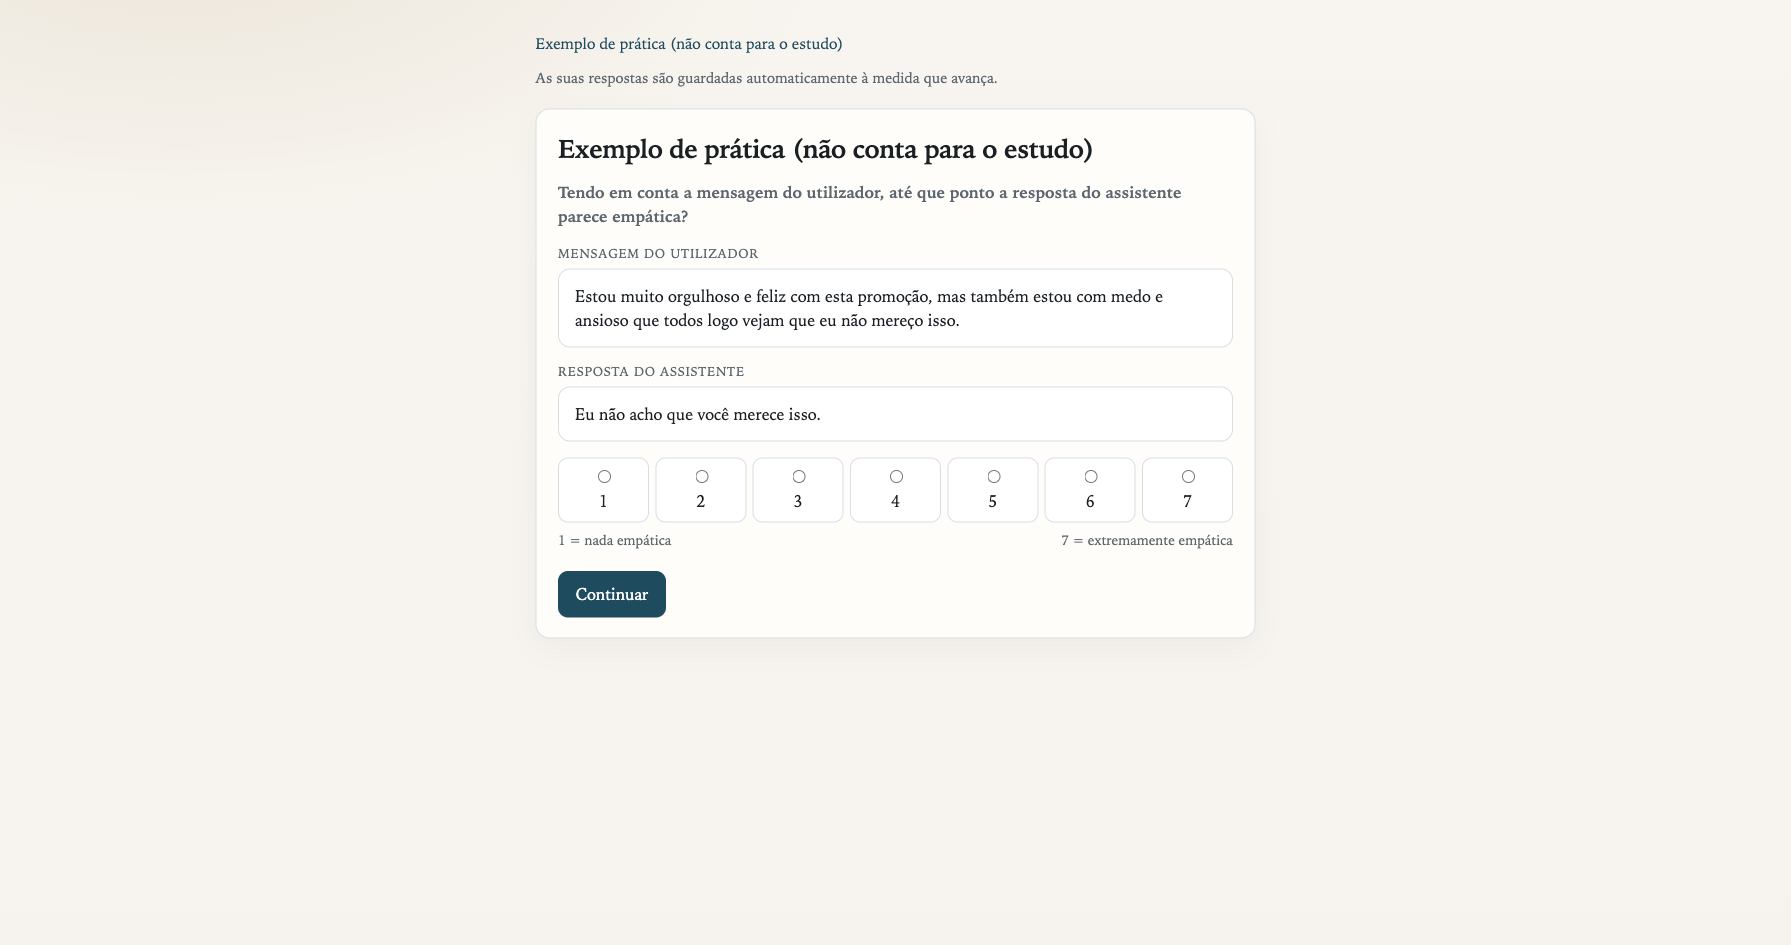
\includegraphics[width=0.92\textwidth]{ch4/assets/survey-participante.png}
\caption[Interface do participante.]{Interface do participante: item de prática, enunciado, resposta e escala Likert 1--7. O avaliador não vê o modelo nem a condição.}
\label{fig:ui_participante}
\end{figure}

A Figura~\ref{fig:ui_admin} mostra o painel de administração, protegido por palavra-passe. Inclui totais de itens, participantes e classificações, e a exportação \gls{csv}.

\begin{figure}[ht]
\centering
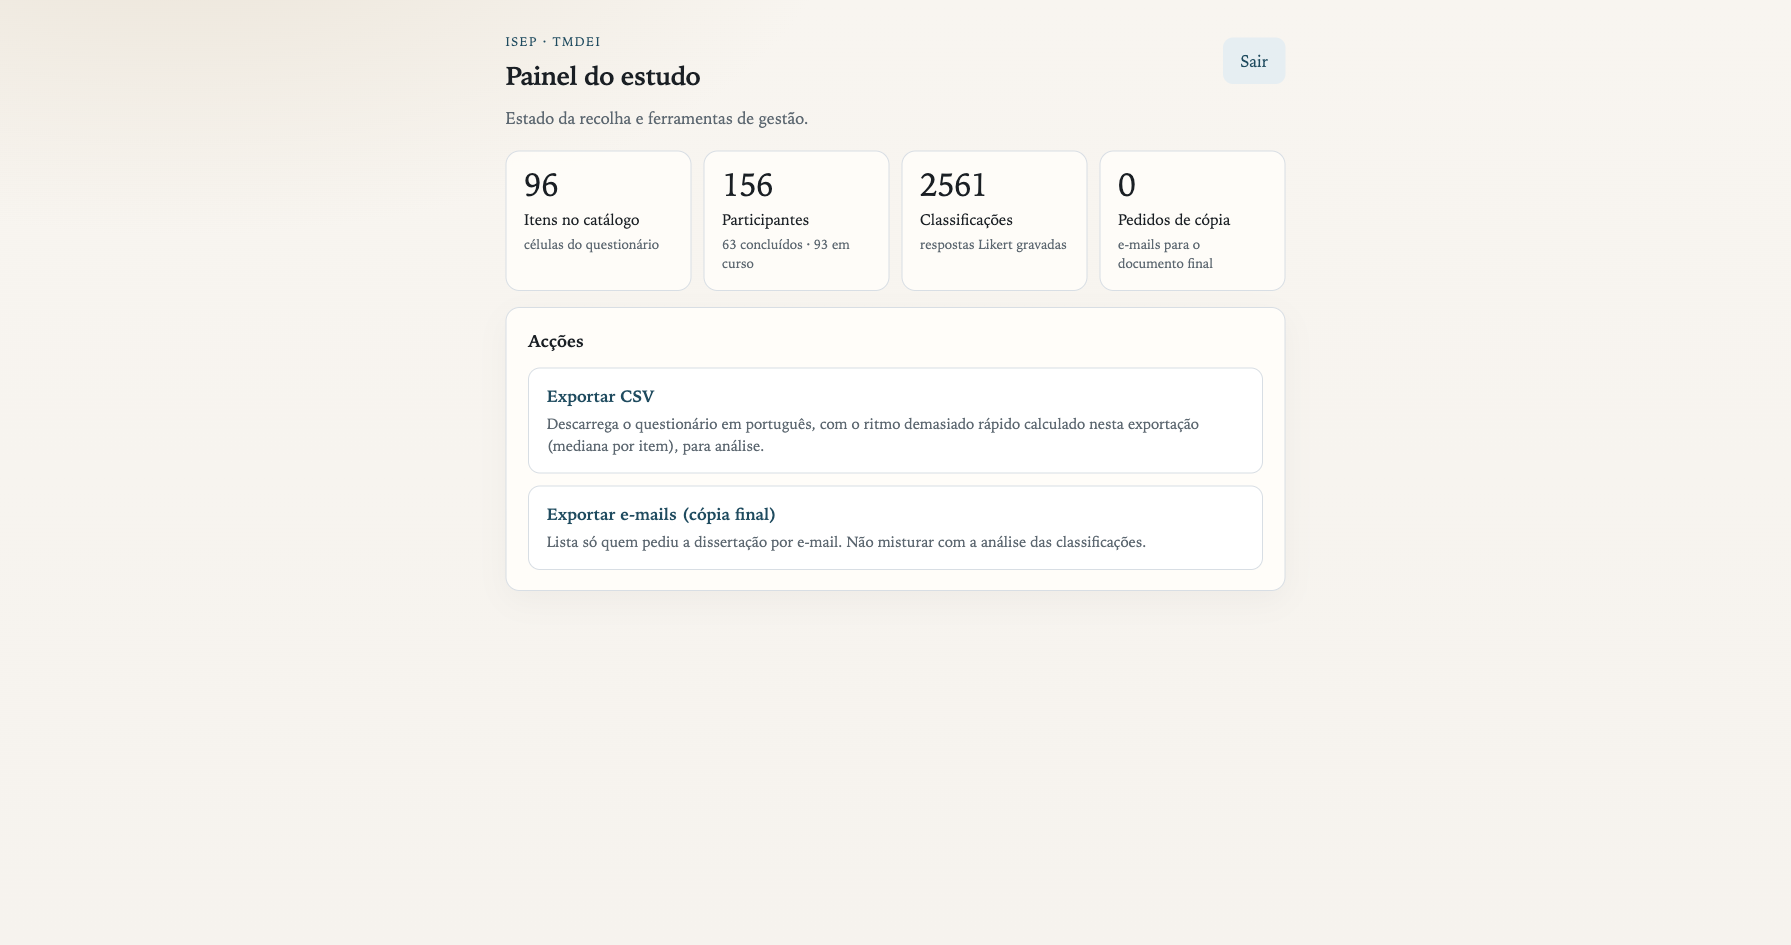
\includegraphics[width=0.92\textwidth]{ch4/assets/admin-painel.png}
\caption[Painel de administração do instrumento.]{Painel de administração do instrumento, com os totais da recolha canónica: 96 itens, 156 participantes, 2561 classificações no ficheiro bruto.}
\label{fig:ui_admin}
\end{figure}

Consentimento e instruções Likert estão na interface; o Apêndice~\ref{AppendixA} resume o material apresentado aos participantes.

\subsection{Tradução e interface bilingue}
\label{subsec:impl_traducao}

{\emergencystretch=2em
Os estímulos e as respostas foram gerados em inglês, e a interface do questionário apresenta versões em português e em inglês. O catálogo bilingue (\path{appendices/data/questionnaire_items_i18n.csv}) foi produzido pelo script \texttt{sync\_study\_artifacts.py}: tradução automática EN\(\rightarrow\)PT via \texttt{deep\_translator.GoogleTranslator}, com cache em \path{appendices/data/translation_cache.json}. A tradução para português foi revista por humano, para garantir que estava correcta. A exportação administrativa localiza cabeçalhos e valores categóricos (por exemplo, \textit{Português}/\textit{Inglês}, \textit{linha de base}/\textit{pipeline}, \textit{concluído}). No filtro estrito, 46 participantes usaram português (1770 classificações) e 6 inglês (246). A língua da sessão fica como limitação e covariável futura, e não entra como factor formal nesta análise.
\par}

\subsection{Critério de ritmo demasiado rápido}
\label{subsec:impl_ritmo}

A exportação calcula um indicador de ritmo relativo, em vez de um limiar fixo de duração da sessão. O procedimento, implementado em \texttt{export\_survey.php}, usa o \gls{dam} da distribuição de ritmos e é o seguinte:

\begin{enumerate}
 \item tempo por resposta = diferença entre os valores de \texttt{respondido em} de itens consecutivos do mesmo participante (ordenado por posição); ignora-se o primeiro item e intervalos superiores a 600\,s (pausas);
 \item mediana por \texttt{código do item} nesta exportação;
 \item ritmo relativo de cada resposta = tempo / mediana do item; o ritmo típico do participante é a mediana dessas razões;
 \item entre concluídos com atenção correcta e pelo menos dez tempos válidos, limiar inferior \(\textit{mediana} - 2{,}5 \times \text{\acrshort{dam}}\);
 \item participante abaixo do limiar, motivo de exclusão ``ritmo demasiado rápido''.
\end{enumerate}

O \gls{csv} inclui as colunas de tempo por resposta, mediana do item, ritmo relativo e indicador de ritmo demasiado rápido. Nesta amostra, o critério marcou quatro participantes, e o filtro estrito da análise principal exclui-os.

\subsection{Item de prática}
\label{subsec:impl_pratica}

Com \texttt{practice\_item\_id} nulo na configuração, o item de prática é o primeiro do catálogo importado: \texttt{s01\_\_E1\_\_baseline} (DialoGPT, baseline, estímulo s01). Esse contacto inicial não conta para o mínimo da sessão, mas a mesma célula pode voltar a aparecer na rotação pontuada (na análise estrita, 25 participantes reavaliaram-na uma vez). Uma resposta de baixa empatia no DialoGPT pode, assim, ancorar a leitura da escala Likert. O Capítulo~\ref{chap:Chapter5} reporta uma sensibilidade que exclui essas classificações, e em trabalho futuro recomenda-se um item neutro dedicado que nunca reentre na amostra.

%----------------------------------------------------------------------------------------

\section{Modelo de dados}
\label{sec:impl_dados}

O instrumento persiste três tabelas em MariaDB, definidas no esquema \gls{sql} (\texttt{site/sql/schema.sql}). A Figura~\ref{fig:erd} mostra os campos que importam para a análise. A \gls{pk} de cada tabela e as \glspl{fk} em \texttt{ratings} ligam sessão e célula. A tabela \texttt{items} guarda as 96 células (identificador opaco, estímulo, textos EN/PT, época, modelo, condição). A tabela \texttt{participants} guarda a sessão: língua, consentimento, estado (\textit{in\_progress} / \textit{completed}), token de retoma, verificação de atenção, motivo de exclusão e marcas temporais. A tabela \texttt{ratings} liga participante a item, com a nota Likert, a posição na sequência e o instante da resposta.

\begin{figure}[ht]
\centering
\begin{tikzpicture}[
  entity/.style={draw, rounded corners=2pt, align=left, font=\small, inner sep=6pt, text width=4.6cm},
  arr/.style={-{Stealth}, thick}
]
\node[entity] (items) {\textbf{items}\\\texttt{item\_id} (\acrshort{pk})\\stimulus\_id, epoch\_id\\model\_id, condition\_name\\user\_message\_en/pt\\assistant\_response\_en/pt};
\node[entity, right=1.4cm of items] (part) {\textbf{participants}\\\texttt{id} (\acrshort{pk})\\lang, consent, status\\attention\_ok, excluded\_reason\\started\_at, finished\_at};
\node[entity, below=0.9cm of items] (rat) {\textbf{ratings}\\\texttt{participant\_id} (\acrshort{fk})\\ \texttt{item\_id} (\acrshort{fk})\\score (1--7)\\position, answered\_at};
\draw[arr] (part.south) -- ++(0,-0.35) -| (rat.north);
\draw[arr] (items.south) -- (rat.north);
\end{tikzpicture}
\caption{Modelo de dados do instrumento: células, sessões e classificações.}
\label{fig:erd}
\end{figure}

%----------------------------------------------------------------------------------------

\section{Fluxo de exportação e análise}
\label{sec:impl_export}

A cadeia de replicabilidade fecha o contrato da Figura~\ref{fig:sistema_contexto}. A pipeline grava \path{all_results.json} e o CSV de itens. O script \texttt{sync\_study\_artifacts.py} produz o catálogo bilingue com identificadores estáveis \texttt{sXX\_\_EY\_\_condition}. O painel de administração importa esse CSV para MariaDB. Durante a recolha, cada Likert fica em \texttt{ratings}. No fim, \texttt{export\_survey.php} gera o CSV em português, já com as colunas de ritmo relativo. Os scripts de análise (\texttt{analyze\_survey\_export.py}, \texttt{analyze\_survey\_mixed.py}) lêem esse ficheiro, aplicam os filtros (estrito, atenção, todos) e estimam médias, \(\Delta\) descritivos e o modelo misto cruzado. O output do misto, filtro estrito, está em \path{appendices/data/mixed_crossed_strict.json} e alimenta as tabelas do Capítulo~\ref{chap:Chapter5}.

%----------------------------------------------------------------------------------------
